\subsection{Automated Configuration Results}
\label{subsec:irace_results}

The automated algorithm configuration process conducted via \texttt{irace} produced five elite metaheuristics on the training set, whose active parameters appear in Table~\ref{tab:irace_elites_vertical}.

\begin{table}[!htbp]
\centering
\resizebox{\linewidth}{!}{
\begin{tabular}{lccccc}
\hline
\textbf{Parameter} & \textbf{$C_1$} & \textbf{$C_2$} & \textbf{$C_3$} & \textbf{$C_4$} & \textbf{$C_5$} \\ \hline
\texttt{initial\_sol} & \texttt{gt} & \texttt{gt} & \texttt{gt} & \texttt{gt} & \texttt{gt} \\ 
\texttt{dispatch\_rule} & \texttt{edd} & \texttt{edd} & \texttt{edd} & \texttt{edd} & \texttt{edd} \\ 
\texttt{search$_1$} & \texttt{ils} & \texttt{ils} & \texttt{ils} & \texttt{ils} & \texttt{ils} \\ 
\texttt{search$_2$} & \texttt{tabu} & \texttt{tabu} & \texttt{tabu} & \texttt{tabu} & \texttt{tabu} \\ 
\texttt{max\_milli\_ils\_iteration} & \texttt{19900} & \texttt{21254} & \texttt{9713} & \texttt{5741} & \texttt{14594} \\ 
\texttt{neighborhood\_number} & \texttt{2} & \texttt{2} & \texttt{3} & \texttt{3} & \texttt{3} \\ 
\texttt{neighborhood$_1$} & \texttt{swap\_penal} & \texttt{swap\_penal} & \texttt{swap\_penal} & \texttt{swap\_rand} & \texttt{swap\_penal} \\ 
\texttt{neighborhood\_exploration$_1$} & \texttt{fi} & \texttt{fi} & \texttt{fi} & \texttt{bi} & \texttt{fi} \\ 
\texttt{neighborhood$_2$} & \texttt{swap\_crit} & \texttt{swap\_crit} & \texttt{swap\_crit} & \texttt{swap\_adj} & \texttt{swap\_crit} \\ 
\texttt{neighborhood\_exploration$_2$} & \texttt{bi} & \texttt{fi} & \texttt{fi} & \texttt{fi} & \texttt{fi} \\ 
\texttt{neighborhood$_3$} & \texttt{-} & \texttt{-} & \texttt{swap\_rand} & \texttt{swap\_penal} & \texttt{swap\_rand} \\ 
\texttt{neighborhood\_exploration$_3$} & \texttt{-} & \texttt{-} & \texttt{fi} & \texttt{bi} & \texttt{fi} \\ 
\texttt{scheduler} & \texttt{linear} & \texttt{linear} & \texttt{linear} & \texttt{linear} & \texttt{linear} \\ 
\texttt{max\_d} & \texttt{29} & \texttt{19} & \texttt{44} & \texttt{65} & \texttt{38} \\ 
\texttt{max\_c} & \texttt{10} & \texttt{2} & \texttt{3} & \texttt{3} & \texttt{2} \\ 
\texttt{tenure} & \texttt{98} & \texttt{96} & \texttt{98} & \texttt{70} & \texttt{85} \\ 
\texttt{elite\_list\_size} & \texttt{23} & \texttt{22} & \texttt{21} & \texttt{13} & \texttt{21} \\ 
\texttt{limit\_iters} & \texttt{2788} & \texttt{2164} & \texttt{1935} & \texttt{2749} & \texttt{1353} \\ 
\texttt{decrease\_divisor} & \texttt{16} & \texttt{12} & \texttt{8} & \texttt{10} & \texttt{11} \\ \hline
\end{tabular}
}
\caption{Parameter configurations of the top five elite algorithms generated by \texttt{irace}.}
\label{tab:irace_elites_vertical}
\end{table}



Cross-configuration analysis reveals that all five elites converge to the same high-level architecture: Giffler--Thompson initialization with EDD, an Iterated Local Search outer loop nesting Tabu Search, and the linear-time right-shift scheduler.
This structural consensus indicates that these components are indispensable for competitive performance in JITJSS.

Regarding neighborhood operators, \texttt{swap\_penal} appears in all five elites (100\%), while \texttt{swap\_crit} is selected in four (80\%). This co-occurrence confirms the synergy between local penalty-aware adjustments \citep{wang2014variable} and structural critical-path reordering.
Conversely, \texttt{irace} eliminated insertion operators and the exact \texttt{relax} neighborhood, favoring lightweight swap moves with lower per-evaluation computational cost.
In terms of overall architecture, the elite configurations represent a hybrid Iterated Tabu Search (ITS) with a multi-neighborhood cyclic VNS progression, combining multiple neighborhood operators with different exploration modes.

To quantify structural convergence across configuration iterations rigorously, we evaluated pairwise configuration dissimilarity using Gower's General Distance Coefficient \citep{gower1971general} alongside the Jaccard Distance Index \citep{jaccard1901etude}.
Gower's distance measures overall dissimilarity across mixed categorical and numerical parameter spaces according to Equation~\eqref{eq:gower}:

\begin{equation} \label{eq:gower}
    d(i,j) = \frac{\sum_{k=1}^n \delta_{ij}^{(k)} s_{ij}^{(k)}}{\sum_{k=1}^n \delta_{ij}^{(k)}}
\end{equation}

where $n$ is the total parameter count, $\delta_{ij}^{(k)} = 1$ if parameter $k$ is active in both configurations (0 otherwise), and $s_{ij}^{(k)}$ is the normalized score: $s_{ij}^{(k)} = 0$ for matching categorical values (1 otherwise), and $s_{ij}^{(k)} = |x_{ik} - x_{jk}| / R_k$ for numerical parameters with domain range $R_k$.

Because Gower's distance evaluates parameter positions independently, it can overestimate dissimilarity when two configurations select identical neighborhood sets in different permutation orders.
Due to the cyclic progression of our VNS container, different permutations of the same neighborhood set exhibit functionally equivalent search behavior.
To complement Gower's metric, we compute the Jaccard Distance Index \citep{jaccard1901etude} over active neighborhood sets $U$ and $V$, evaluating set-level dissimilarity independently of derivation order according to Equation~\eqref{eq:jaccard}:

\begin{equation} \label{eq:jaccard}
    Jaccard(U,V) = 1 - \frac{|U \cap V|}{|U \cup V|}
\end{equation}

Figure~\ref{fig:grafico_variancia} tracks the average pairwise Gower and Jaccard distances across all 11 \texttt{irace} configuration iterations.
Both metrics decrease sharply over the first iterations before stabilizing, showing that \texttt{irace} rapidly discarded uncompetitive regions and converged toward a stable, high-performing consensus area.


\begin{figure}[!htbp] 
    \centering 
    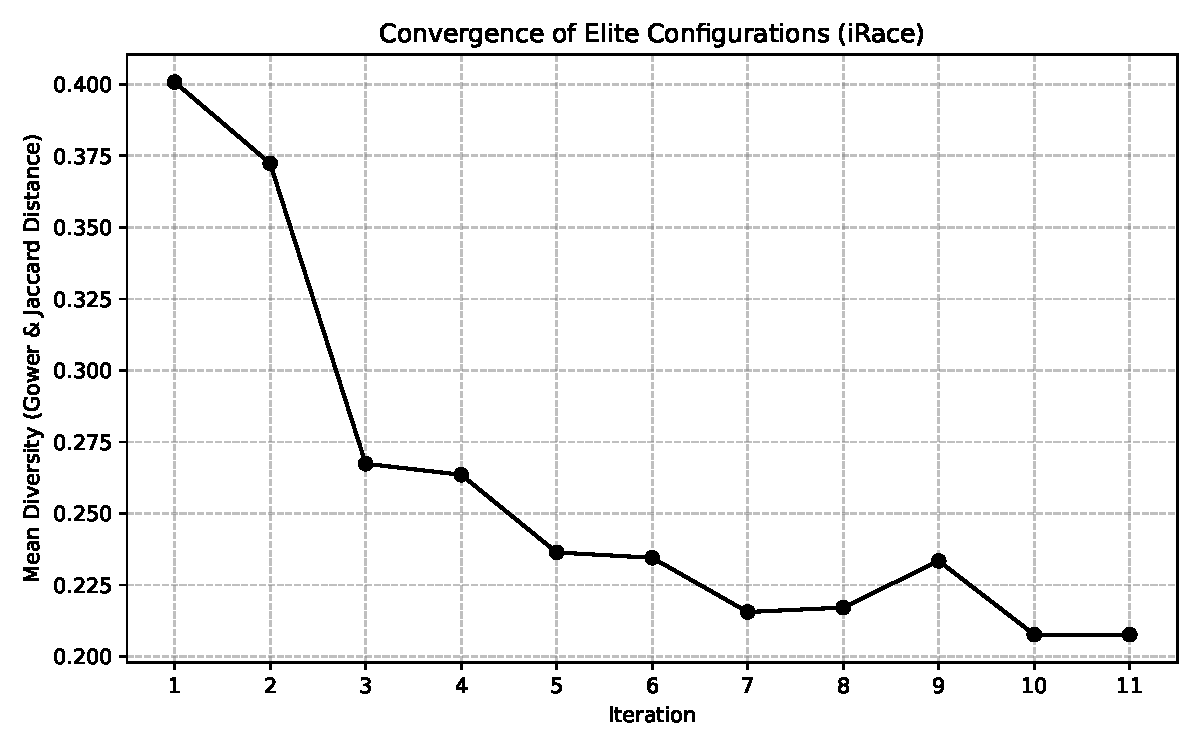
\includegraphics[width=0.85\linewidth]{img/config_convergence.pdf}
    % \caption{Evolution of average pairwise Gower and Jaccard distances among elite configurations across \texttt{irace} iterations.}
    \caption{\textbf{Structural and parametric diversity convergence of elite configurations throughout \texttt{irace} iterations.} 
    The curve depicts the evolution of the average pairwise distance among candidate configurations retained in the elite pool across consecutive racing iterations. Categorical structural choices (e.g., search strategies, dispatching rules, and neighborhood types) are assessed via Jaccard distance, while numerical hyperparameters are evaluated using Gower distance, illustrating the progressive transition from broad design-space exploration to exploitation and final convergence.}
    \label{fig:grafico_variancia}
\end{figure}

\subsection{Literature Benchmark Results}
\label{subsec:benchmark_tests}

We evaluated the generalization performance of the five elite configurations on the 72 standard JITJSS benchmark instances of \citet{baptiste2008lagrangian}.
Performance is benchmarked against the Best-Known Solutions (BKS), defined as the minimum objective value across the five state-of-the-art studies: \citet{dos2010combination}, \citet{wang2014variable}, \citet{ahmadian2021meta}, \citet{abderrazzak2022adaptive}, and \citet{sabri2023reinforcement}.
Because the algorithms incorporate stochastic search components, each configuration was executed 5 times per instance using 5 distinct random seeds.


To ensure a rigorous and fair computational comparison against the state-of-the-art baseline of \citet{ahmadian2021meta}, we standardized runtime budgets across problem scales using single-thread CPU benchmark scores from PassMark.
The reference experiments of \citet{ahmadian2021meta} were executed on a processor rated at 2,088 single-thread PassMark points, with average runtimes of 47, 119, and 250 seconds for instances with 10, 15, and 20 jobs, respectively.
Adjusting these durations for our hardware (rated at 2,762 points, yielding a speedup ratio of $2088 / 2762 \approx 0.756$) would correspond to equivalent execution times of roughly 35.5, 90.0, and 189.0 seconds.
To provide a strictly conservative evaluation margin in favor of the literature baseline, we bounded our algorithm's maximum execution time to 25, 75, and 150 seconds for $n \in \{10, 15, 20\}$, respectively.

Because the Iterated Local Search (ILS) framework executes until reaching its allocated time budget, these limits serve as the outer stopping criterion.
Crucially, our framework logs the exact timestamp at which each global best solution is discovered.
While all runs exhausted their allocated budgets, configuration $C_1$ converged to its final best solutions in an average of 3.7, 20.7, and 61.4 seconds for instances with 10, 15, and 20 jobs, respectively, demonstrating that high-quality schedules are identified well before the conservative time horizons expire.


% \begin{table}[ht]
\centering
\caption{Computational results of configuration C1 for instances with 10 jobs.}
\label{tab:results_10}
\resizebox{\textwidth}{!}{
\begin{tabular}{lcccccccc}
\hline
\textbf{Instance}                & \textbf{Cplex}           & \textbf{[1]}          & \textbf{[2]}            & \textbf{[3]}        & \textbf{[4]}       & \textbf{[5]}        & \textbf{$B$} & \textbf{$M$}  \\
\hline
loose-equal-1-10x2  & \textbf{224.84} & \textbf{224.84} & \textbf{224.84} & \textbf{224.84} & \textbf{224.84} & \textbf{224.84}    & \textbf{224.84}       & \textbf{224.84}         \\
loose-equal-2-10x2  & \textbf{319.37} & 324.43          & \textbf{319.37} & \textbf{319.37} & \textbf{319.37} & \textbf{319.37}    & \textbf{319.37}       & \textbf{319.37}         \\
loose-equal-1-10x5  & 1738.05         & 1733.38         & 1738.05         & \textbf{1719.63} & 1725.16         & \textbf{1719.63}  & \textbf{1719.63}      & 1738.63                \\
loose-equal-2-10x5  & 971.96          & 968.89          & \textbf{967.73} & \textbf{967.73} & 968.05          & \textbf{967.73}    & \textbf{967.63}       & \textbf{967.73}                  \\
loose-equal-1-10x10 & 360.74          & 366.77          & 365.81          & 364.39          & 360.56          & \textbf{360.33}    & 360.74                & 364.59                  \\
loose-equal-2-10x10 & 251.86          & \textbf{249.85} & 252.99          & \textbf{249.85} & \textbf{249.85} & \textbf{249.85}    & \textbf{249.85}       & \textbf{249.85}         \\
loose-tard-1-10x2   & \textbf{416.44} & \textbf{416.44} & \textbf{416.44} & \textbf{416.44} & \textbf{416.44} & \textbf{416.44}    & \textbf{416.44}       & \textbf{416.44}         \\
loose-tard-2-10x2   & \textbf{137.94} & \textbf{137.94} & \textbf{137.94} & \textbf{137.94} & \textbf{137.94} & \textbf{137.94}    & \textbf{137.94}       & \textbf{137.94}         \\
loose-tard-1-10x5   & 176.83          & \textbf{175.08} & \textbf{175.08} & \textbf{175.08} & \textbf{175.08} & \textbf{175.08}    & \textbf{175.08}       & \textbf{175.08}                  \\
loose-tard-2-10x5   & 492.05          & 525.88          & 499.93          & \textbf{485.06} & 488.6           & 486.93             & \textbf{485.06}       & \textbf{485.06}         \\
loose-tard-1-10x10  & 375.71          & 383.84          & 380.26          & \textbf{374.2}  & \textbf{374.2}  & 375.58             & \textbf{374.2}        & 386.4                  \\
loose-tard-2-10x10  & \textbf{144.94} & \textbf{144.94} & 144.99          & \textbf{144.94} & \textbf{144.94} & \textbf{144.94}    & \textbf{144.94}       & \textbf{144.94}         \\
tight-equal-1-10x2  & \textbf{461.96} & \textbf{461.96} & \textbf{461.96} & \textbf{461.96} & \textbf{461.96} & \textbf{461.96}    & \textbf{461.96}       & \textbf{461.96}         \\
tight-equal-2-10x2  & \textbf{448.32} & \textbf{448.32} & \textbf{448.32} & \textbf{448.32} & \textbf{448.32} & \textbf{448.32}    & \textbf{448.32}       & \textbf{448.32}         \\
tight-equal-1-10x5  & \textbf{689.11} & \textbf{689.11} & \textbf{689.11} & \textbf{689.11} & \textbf{689.11} & \textbf{689.11}    & \textbf{689.11}       & 690.29                  \\
tight-equal-2-10x5  & \textbf{763.24} & 770.49          & 764.03          & \textbf{763.24} & \textbf{763.24} & \textbf{763.24}    & \textbf{763.24}       & \textbf{763.24}         \\
tight-equal-1-10x10 & 1281.66         & \textbf{1276.23} & 1277.44         & \textbf{1276.23} & \textbf{1276.23} & 1279.82         & 1281.66      & 1301.46                 \\
tight-equal-2-10x10 & 1885.25         & 1885.25         & 1871.23         & 1866.92         & 1865.94 & 1886.93                    & \textbf{1865.93}      & 1873.64                 \\
tight-tard-1-10x2   & \textbf{179.46} & \textbf{179.46} & \textbf{179.46} & \textbf{179.46} & \textbf{179.46} & \textbf{179.46}    & \textbf{179.46}       & \textbf{179.46}         \\
tight-tard-2-10x2   & \textbf{145.37} & \textbf{145.37} & \textbf{145.37} & \textbf{145.37} & \textbf{145.37} & \textbf{145.37}    & \textbf{145.37}       & \textbf{145.37}         \\
tight-tard-1-10x5   & \textbf{379.19} & 380.82          & 380             & \textbf{379.19} & \textbf{379.19} & \textbf{379.19}    & 386.57                & 389.43                  \\
tight-tard-2-10x5   & 635.93          & \textbf{627.45} & 628.68          & \textbf{627.45} & 628.02          & \textbf{627.45}    & \textbf{627.45}       & \textbf{627.45}         \\
tight-tard-1-10x10  & 687.65          & 717.85          & 746.03          & 668.14          & \textbf{667.97} & 669.15             & 669.93                & 687.65                  \\
tight-tard-2-10x10  & 779.17          & 780.82          & 785.79          & \textbf{777.85} & 778.32          & 780.74             & 780.66                & 804.23                  \\
\hline
\end{tabular}
}
\end{table}

%
% \begin{table}[ht]
\centering
\caption{Computational results of configuration C1 for instances with 15 jobs.}
\label{tab:results_15}
\resizebox{\textwidth}{!}{
\begin{tabular}{lcccccccc}
\hline
\textbf{Instance}                & \textbf{Cplex}           & \textbf{[1]}          & \textbf{[2]}            & \textbf{[3]}        & \textbf{[4]}       & \textbf{[5]}        & \textbf{$B$} & \textbf{$M$}   \\
\hline
loose-equal-1-15x2  & \textbf{1041.33} & \textbf{1041.33} & \textbf{1041.33} & \textbf{1041.33} & \textbf{1041.33} & \textbf{1041.33} & \textbf{1041.33}    & \textbf{1041.33}  \\
loose-equal-2-15x2  & \textbf{497.97}  & \textbf{497.97}  & 514.72          & 512.54          & \textbf{497.97}  & \textbf{497.97}    & \textbf{497.97}     & 505.16           \\
loose-equal-1-15x5  & 3457.57         & 3220.16         & 3321.54         & 3272.46         & 3258.72         & 3229.16               & \textbf{3196.85}    & 3247.89  \\
loose-equal-2-15x5  & 3437.32         & 3328.86         & 3310.27         & 3260.81         & 3255.13         & \textbf{3251.84}      & 3274.38             & 3290.70                 \\
loose-equal-1-15x10 & \textbf{875.74}  & 1008.28         & 977.43          & 906.49          & 897.51          & 913.26               & 898.99              & 938.80                \\
loose-equal-2-15x10 & 1587.09         & 1720.18         & 1584.44         & \textbf{1487.33} & 1538.27         & 1492.11              & 1554.18             & 1594.60                \\
loose-tard-1-15x2   & \textbf{654.84}  & \textbf{654.84}  & \textbf{654.84}  & \textbf{654.84}  & \textbf{654.84}  & \textbf{654.84}  & \textbf{654.84}     & \textbf{654.84}   \\
loose-tard-2-15x2   & 293.17          & \textbf{279.71}  & 297.54          & 285.16          & 289.36          & \textbf{279.71}      & \textbf{279.71}     & 290.88           \\
loose-tard-1-15x5   & 1281.87         & 1320.93         & 1315.47         & 1281    & 1292.28         & 1317.56                       & \textbf{1280.74}    & 1281.41          \\
loose-tard-2-15x5   & 335.55          & 329.47          & 335.55          & 328.26  & 330.14          & 332.25                        & \textbf{327.60}     & 328.88           \\
loose-tard-1-15x10  & \textbf{277}     & 297.19          & 296.6           & \textbf{277}     & \textbf{277}     & \textbf{277}       & 281.45              & 287.03              \\
loose-tard-2-15x10  & 597.93  & 713.97          & 664.13          & 601.24          & 627.81          & 603.67                        & \textbf{587.24}     & \textbf{592.31}         \\
tight-equal-1-15x2  & 3366.66         & \textbf{3344.54} & \textbf{3344.54} & \textbf{3344.54} & \textbf{3344.54} & \textbf{3344.54}  & \textbf{3344.54}    & \textbf{3344.54}   \\
tight-equal-2-15x2  & \textbf{1479.76} & \textbf{1479.76} & \textbf{1479.76} & \textbf{1479.76} & \textbf{1479.76} & \textbf{1479.76} & \textbf{1479.76}    & \textbf{1479.76}   \\
tight-equal-1-15x5  & 1412.71         & 1369.06         & 1345.21         & 1342.3          & 1343.08         & 1345.18               & \textbf{1318.68}    & \textbf{1318.68}   \\
tight-equal-2-15x5  & 2782.17         & 2630.06         & 2709.13         & 2641.28         & \textbf{2563.16} & 2602.99               & 2626.67             & 2651.16           \\
tight-equal-1-15x10 & 7167.59         & 7380.76         & 8120.43         & 6820.87         & 6811.54 & 7115.63                       & \textbf{6610.44}    & \textbf{6748.88}           \\
tight-equal-2-15x10 & 5407.42         & 4893.44         & 4966.34         & 4760.48         & 4801.47         & 4757.06                & \textbf{4652.41}    & \textbf{4730.08}    \\
tight-tard-1-15x2   & 806.92          & \textbf{790.5}   & 790.66          & \textbf{790.5}   & \textbf{790.5}   & \textbf{790.5}     & \textbf{790.5}      & \textbf{790.5}       \\
tight-tard-2-15x2   & \textbf{905.37}  & \textbf{905.37}  & \textbf{905.37}  & \textbf{905.37}  & \textbf{905.37}  & \textbf{905.37}   & \textbf{905.37}     & \textbf{905.37}      \\
tight-tard-1-15x5   & 1371.29         & 1371.37         & 1426.97         & 1359.18         & 1366.45         & \textbf{1341.69}       & 1358.21             & 1359.18            \\
tight-tard-2-15x5   & 721.46          & 691.1           & 725.72          & 681.27          & 677.8           & 695.08                 & \textbf{677.57}     & 681.62     \\
tight-tard-1-15x10  & 815.03          & 800.87          & 832.08          & 767.26  & 770.91          & 775.4                          & \textbf{757.83}     & 785.75        \\
tight-tard-2-15x10  & 1267.53         & 1310.04         & 1452.9          & 1224.82         & 1243.52         & 1226.23                & \textbf{1170.94}    & \textbf{1172.30}     \\
\hline
\end{tabular}
}
\end{table}

%
% \begin{table}[ht]
\centering
\resizebox{\textwidth}{!}{
\begin{tabular}{lcccccccc}
\hline

\textbf{Instance}                & \textbf{Cplex}           & \textbf{D}          & \textbf{W}            & \textbf{A}        & \textbf{$B$} & \textbf{$M$}  \\
\hline
loose-equal-1-20x2 & 2565.51 & 2548.95 & 2551.22 & 2548.95 & \textbf{2547.92} & \textbf{2548.95} \\
loose-equal-2-20x2 & 3105.34 & \textbf{3069.13} & 3070.16 & \textbf{3069.13} & \textbf{3069.13} & \textbf{3069.13} \\
loose-equal-1-20x5 & 8271.34 & 7545.44 & 7758.02 & 7524.13 & \textbf{7487.77} & 7649.11 \\
loose-equal-2-20x5 & 7793.45 & 7252.81 & 7302.01 & 7059.38 & \textbf{7008.65} & 7086.24 \\
loose-equal-1-20x10 & 5597.4 & 5260.48 & 5476.47 & 4651.31 & \textbf{4507.31} & 4665.08 \\
loose-equal-2-20x10 & 1862.41 & 1987.65 & 1718.08 & \textbf{1597.89} & 1608.14 & 1659.73 \\
loose-tard-1-20x2 & 1265.36 & 1206.97 & 1205.59 & 1206.4 & \textbf{1203.88} & \textbf{1204.43} \\
loose-tard-2-20x2 & 772.89 & \textbf{769.35} & 790.12 & \textbf{769.35} & 771.06 & 782.39 \\
loose-tard-1-20x5 & 3548.14 & 2938.24 & 3517.2 & 2931.11 & \textbf{2874.65} & 2937.00 \\
loose-tard-2-20x5 & 4048.77 & 3722.61 & 3684.67 & 3627.51 & \textbf{3615.47} & 3643.19 \\
loose-tard-1-20x10 & 6494.34 & 5093.89 & 5478.21 & 4817.32 & \textbf{4775.01} & 5094.21 \\
loose-tard-2-20x10 & 1545.95 & 1570.64 & 1599.55 & \textbf{1401.28} & 1502.23 & 1530.81 \\
tight-equal-1-20x2 & 1940.06 & 1937.49 & 1939.11 & 1936.45 & \textbf{1933.72} & \textbf{1933.72} \\
tight-equal-2-20x2 & 961.44 & \textbf{941.69} & 959.65 & 943.7 & 948.01 & 948.01 \\
tight-equal-1-20x5 & 3013.79 & 2866.94 & 2935.95 & 2865.95 & \textbf{2821.00} & 2868.29 \\
tight-equal-2-20x5 & 7233.35 & 6741.16 & 6964.91 & 6613.62 & \textbf{6581.72} & 6617.41 \\
tight-equal-1-20x10 & 11561.7 & 10607.2 & 11073.1 & \textbf{10378.8} & 10534.50 & 10813.10 \\
tight-equal-2-20x10 & 8501.42 & 7310.32 & 7317.74 & \textbf{6839.3} & 6876.49 & 6955.14 \\
tight-tard-1-20x2 & 1675.37 & \textbf{1671.87} & 1682.94 & 1674.6 & \textbf{1671.87} & \textbf{1671.87} \\
tight-tard-2-20x2 & 1489.65 & \textbf{1448.66} & 1459.57 & 1451.61 & \textbf{1448.66} & \textbf{1448.66} \\
tight-tard-1-20x5 & 3821.29 & 3672.18 & 3669.09 & 3620.61 & \textbf{3598.12} & \textbf{3618.13} \\
tight-tard-2-20x5 & 1881.02 & 1858.19 & 1976.11 & 1792.78 & \textbf{1784.19} & 1808.36 \\
tight-tard-1-20x10 & 4984.31 & 4853.81 & 5536.64 & 4445.59 & \textbf{4309.35} & \textbf{4434.02} \\
tight-tard-2-20x10 & 4057.01 & 3358.61 & 3245.9 & \textbf{3085.54} & 3196.75 & 3239.89 \\
\hline
\end{tabular}
}
\caption{Computational results of configuration C1 for instances with 20 jobs.Literature sources: D (\citet{dos2010combination}), W (\citet{wang2014variable}), Cplex and A (\citet{ahmadian2021meta}).}
\label{tab:results_20}
\end{table}


\begin{table}[!htbp]
\centering
\resizebox{0.95\linewidth}{!}{
\begin{tabular}{lccccc}
\hline
\textbf{Performance Metric} & \textbf{$C_1$} & \textbf{$C_2$} & \textbf{$C_3$} & \textbf{$C_4$} & \textbf{$C_5$} \\ \hline
Instances where Best solution ($B$) $\le$ BKS & 52 & 47 & 47 & 41 & 49 \\ 
Instances where Median solution ($M$) $\le$ BKS & 35 & 29 & 33 & 32 & 28 \\ 
\hline
\end{tabular}
}
\caption{Performance summary of the five elite configurations on the 72 benchmark test instances.}
\label{tab:results_confs}
\end{table}



Table~\ref{tab:results_confs} summarizes performance across the test set, reporting the count of instances where the best ($B$) and median ($M$) solutions over five runs matched or improved the BKS.
Configuration $C_1$ attained the highest success rate across both metrics, matching or improving the BKS in 72.2\% (best) and 48.6\% (median) of instances; we thus select it as the representative algorithm for detailed comparison.

Full instance-by-instance numerical comparisons across all problem scales ($n \in \{10, 15, 20\}$) are documented in \ref{app:detailed_results}.

Across the benchmark suite, $C_1$ matches or improves the BKS in 72.2\% of instances, maintaining high competitiveness across all scales: 70.8\% for $n=10$, 75.0\% for $n=15$, and 70.8\% for $n=20$.
Analysis of median results further confirms algorithmic robustness: across five stochastic runs, the median solution matched or improved upon the literature best in 48.6\% of instances, with an average percentage deviation of only 0.96\% relative to the best individual runs.

\begin{figure}[!htbp] 
    \centering 
    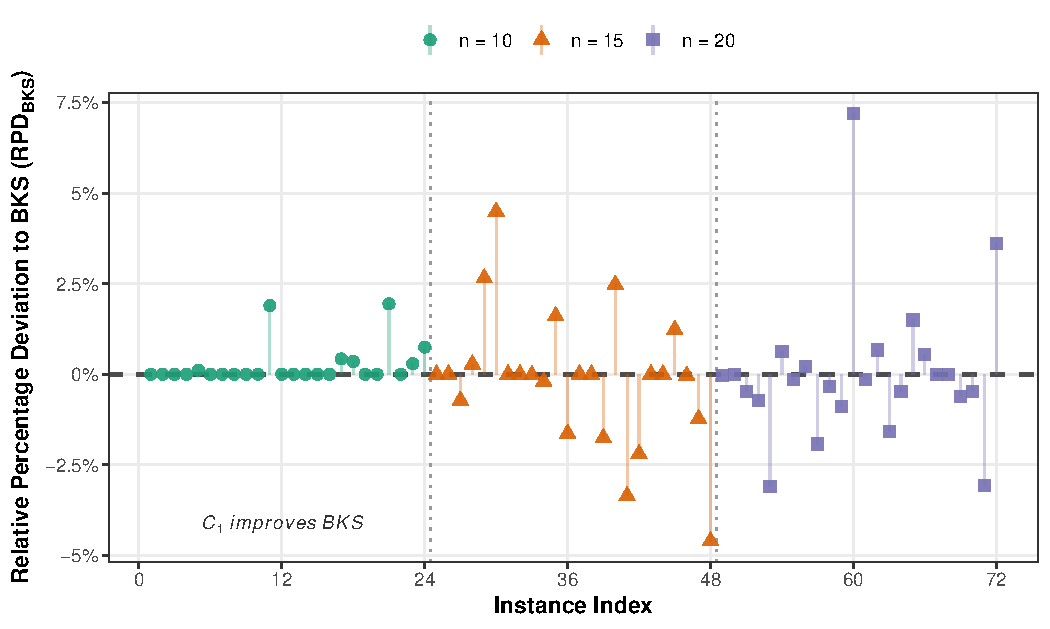
\includegraphics[width=0.75\linewidth]{img/rpd_dispersion_c1.pdf}
    % \caption{Relative Percentage Deviation (RPD) of configuration $C_1$ relative to the literature Best-Known Solutions (BKS) across all 72 benchmark instances. The dashed horizontal line at $0\%$ represents the literature BKS baseline, with negative values indicating strictly improved upper bounds. Vertical dotted lines delimit problem scales ($n \in \{10, 15, 20\}$).}
    \caption{\textbf{Solution quality dispersion of configuration $C_1$ relative to the literature Best-Known Solutions (BKS).} 
    Relative percentage deviations ($\text{RPD}_{\text{BKS}}$) are plotted across all 72 benchmark instances of \citet{baptiste2008lagrangian}, ordered along the horizontal axis. The dashed horizontal line at $0\%$ represents the literature BKS baseline, where negative values indicate instances where $C_1$ established strictly superior upper bounds. Vertical dotted lines partition instances across problem scales ($n=10$, $n=15$, and $n=20$), with distinct point markers and stems indicating individual instance deviations.}
    \label{fig:deviation_disper}
\end{figure}

This consistency is illustrated in Figure~\ref{fig:deviation_disper}, which details the Relative Percentage Deviation (RPD) of $C_1$ with respect to the BKS across all 72 instances.
Points situated on or below the zero-deviation reference line denote instances where $C_1$ matched or strictly improved the current literature bounds, demonstrating that significant cost reductions are achieved systematically across all three problem scales without catastrophic outliers on the harder 20-job instances.

\begin{table}[!htbp]
\centering
\resizebox{0.95\linewidth}{!}{
\begin{tabular}{lccccc}
\hline
\textbf{Baseline} & \textbf{Coverage ($N$)} & \textbf{Success Rate (\%)} & \textbf{$V$} & \textbf{$p$-value} & \textbf{Statistical Verdict} \\ \hline
\citet{dos2010combination}     & 72 & 94.4\% & 46  & $9.00 \times 10^{-9}$ & $C_1$ significantly better \\
\citet{wang2014variable}        & 72 & 97.2\% & 39  & $3.06 \times 10^{-10}$ & $C_1$ significantly better \\
\citet{ahmadian2021meta}        & 72 & 77.7\% & 353 & 0.01295               & $C_1$ significantly better \\ \hline
\citet{abderrazzak2022adaptive} & 48 & 79.1\% & 146 & 0.09912               & Statistically comparable \\
\citet{sabri2023reinforcement}  & 48 & 81.2\% & 97  & 0.06681               & Statistically comparable \\ \hline
\end{tabular}
}
\caption{Pairwise performance comparison and Wilcoxon signed-rank tests between configuration $C_1$ and literature baselines (one-tailed, alternative: $C_1 < \text{baseline}$, $\alpha = 0.05$).}
\label{tab:comparacao_estado_wilcoxon}
\end{table}


Table~\ref{tab:comparacao_estado_wilcoxon} summarizes the pairwise comparisons and one-tailed Wilcoxon signed-rank tests against each baseline.
Across the complete set of 72 instances, $C_1$ matches or improves upon \citet{dos2010combination} (94.4\%), \citet{wang2014variable} (97.2\%), and \citet{ahmadian2021meta} (77.7\%), with statistically significant differences ($p < 0.05$).
For the 48-instance subset evaluated by \citet{abderrazzak2022adaptive} and \citet{sabri2023reinforcement}, $C_1$ achieves success rates of 79.1\% and 81.2\%, exhibiting statistical comparability ($p = 0.09912$ and $p = 0.06681$) while successfully extending evaluation to the large-scale 20-job instances omitted by both studies.

\begin{table}[!htbp]
\centering
\resizebox{\linewidth}{!}{
\begin{tabular}{lcccc|lcccc}
\hline
\textbf{Instance} & \textbf{Prev. BKS} & \textbf{Source} & \textbf{New BKS} & \textbf{Source Config.} & \textbf{Instance} & \textbf{Prev. BKS} & \textbf{Source} & \textbf{New BKS} & \textbf{Source Config.} \\ \hline
tight-equal-2-10x10 & 1865.94 & AB & 1824.50 & $C_2$ & loose-equal-2-20x5  & 7059.38 & A & 6953.68 & $C_5$\\
loose-equal-1-15x5  & 3220.16 & D  & 3196.85 & $C_1,C_2,C_3,C_4$& loose-equal-1-20x10 & 4651.31 & A & 4507.31 & $C_1$\\
loose-tard-1-15x5   & 1281.00 & A  & 1280.74 & $C_1$& loose-tard-1-20x2   & 1205.59 & W & 1203.88 & $C_1, C_2, C_3, C_4, C_5$\\
loose-tard-2-15x5   & 328.26  & A  & 327.60  & $C_1$& loose-tard-1-20x5   & 2931.11 & A & 2857.91 & $C_4$\\
loose-tard-2-15x10  & 597.93  & A  & 583.23  & $C_2,C_5$& loose-tard-2-20x5   & 3627.51 & A & 3615.47 & $C_1$\\
tight-equal-1-15x5  & 1342.30 & A  & 1318.68 & $C_1,C_2,C_3,C_4,C_5$& loose-tard-1-20x10  & 4817.32 & A & 4775.01 & $C_1$\\
tight-equal-1-15x10 & 6811.54 & AB & 6582.59 & $C_1,C_3,C_5$& tight-equal-1-20x2  & 1936.45 & A & 1933.72 & $C_1, C_2, C_3, C_5$\\
tight-equal-2-15x10 & 4757.06 & S  & 4626.28 & $C_2$& tight-equal-1-20x5  & 2865.95 & A & 2821.00 & $C_1$\\
tight-tard-2-15x5   & 677.80  & AB & 677.57  & $C_1,C_3,C_4,C_5$& tight-equal-2-20x5  & 6613.62 & A & 6581.72 & $C_, C_2$\\
tight-tard-1-15x10  & 767.26  & A  & 757.83  & $C_1$& tight-tard-1-20x5   & 3620.61 & A & 3592.28 & $C_2$\\
tight-tard-2-15x10  & 1224.82 & A  & 1140.85 & $C_5$& tight-tard-2-20x5   & 1792.78 & A & 1784.19 & $C_1$\\
loose-equal-1-20x2  & 2548.95 & D  & 2547.68 & $C_2, C_3, C_4, C_5$& tight-tard-1-20x10  & 4445.59 & A & 4305.08 & $C_3$\\
loose-equal-1-20x5  & 7524.13 & A  & 7487.77 & $C_1,C_3$&                     &         &   &         & \\
\hline
\end{tabular}
}
\caption{New best-known solutions (BKS) established on the \citet{baptiste2008lagrangian} benchmark suite. Literature sources: A (\citet{ahmadian2021meta}), AB (\citet{abderrazzak2022adaptive}), D (\citet{dos2010combination}), S (\citet{sabri2023reinforcement}), and W (\citet{wang2014variable}).}
\label{tab:new_bks}
\end{table}


In addition to the standalone evaluation of configuration $C_1$, we aggregated the solutions discovered across all experimental runs of the elite configurations to identify potential improvements to the benchmark's historical records.
Table~\ref{tab:new_bks} lists the instances where our experiments established new best-known upper bounds, reporting the previous literature reference and the newly discovered objective value.
Across the entire suite, our framework improved the historical BKS in 25 instances, providing tighter upper bounds to support future benchmarking and exact optimization studies for the JITJSS.



